\documentclass[10pt,a4paper,dvipdfmx,uplatex]{jsarticle}
\usepackage{jasmine}

\title{HST/WFC3 の画像を用いたバックグラウンドレベルの推定}
\subtitle{JASMINE-C2-TN-RO-20220330-01-background}

\author{大澤亮}
\date{\today}

\begin{document}
\maketitle

\begin{abstract}
  JASMINE が観測する銀河中心領域における広がったバックグラウンド放射の強度レベルを見積もる. Hubble Legacy Archive (HLA) から銀河中心を赤外線チャンネルで観測したデータを取得し, ヒストグラムからバックグラウンド放射のカウントレートを求めて面輝度に変換する. 2 つの観測プロジェクトから 2 波長合計 16 枚の画像データを取得した. カウント値からエネルギーフラックスに変換して光子のレートに変換する.
\end{abstract}

\section{検討の方針}
JASMINE が観測する銀河中心領域は天体が密に存在しており, 暗い星の重ね合わせによって広がったバックグラウンド放射を構成していると考えられる. 地上観測では点源に分解できなかった放射は前景の大気からの放射と見分けがつかないため, 放射レベルの絶対値を見積もることは難しい. そこで, 宇宙からの観測でありキャリブレーションされたデータが公開されている Hubble Space Telescope の Wide Field Camera 3 (WFC3)\footnote{\url{https://www.stsci.edu/hst/instrumentation/wfc3}}のデータを使用してバックグラウンド放射の強度レベルを見積もる.


\section{使用するデータ}
Hubble Legacy Archive (HLA)\footnote{\url{https://hla.stsci.edu/hla_welcome.html}} で銀河中心から半径 0.5\deg に存在する観測データを検索した. 図~\ref{fig:screen:hla} に HLA のスクリーンショットを表示した. ここでは JASMINE の観測波長域に近い \texttt{F127M} ($\SI{1.274}{\micro\meter}$) と \texttt{F139M} ($\SI{1.384}{\micro\meter}$) のフィルタで観測がされていた 2 つのプロジェクトのデータを取得した. データの諸情報を表\ref{tab:data} にまとめた. いずれのデータもリダクション済みであり, 複数枚の画像の足し合わせや明るさのキャリブレーションも完了している. HLA では \texttt{DAOPHOT} を使用して測光した結果も公開されている. 参考のためこちらもダウンロードした.

\begin{figure}
  \centering
  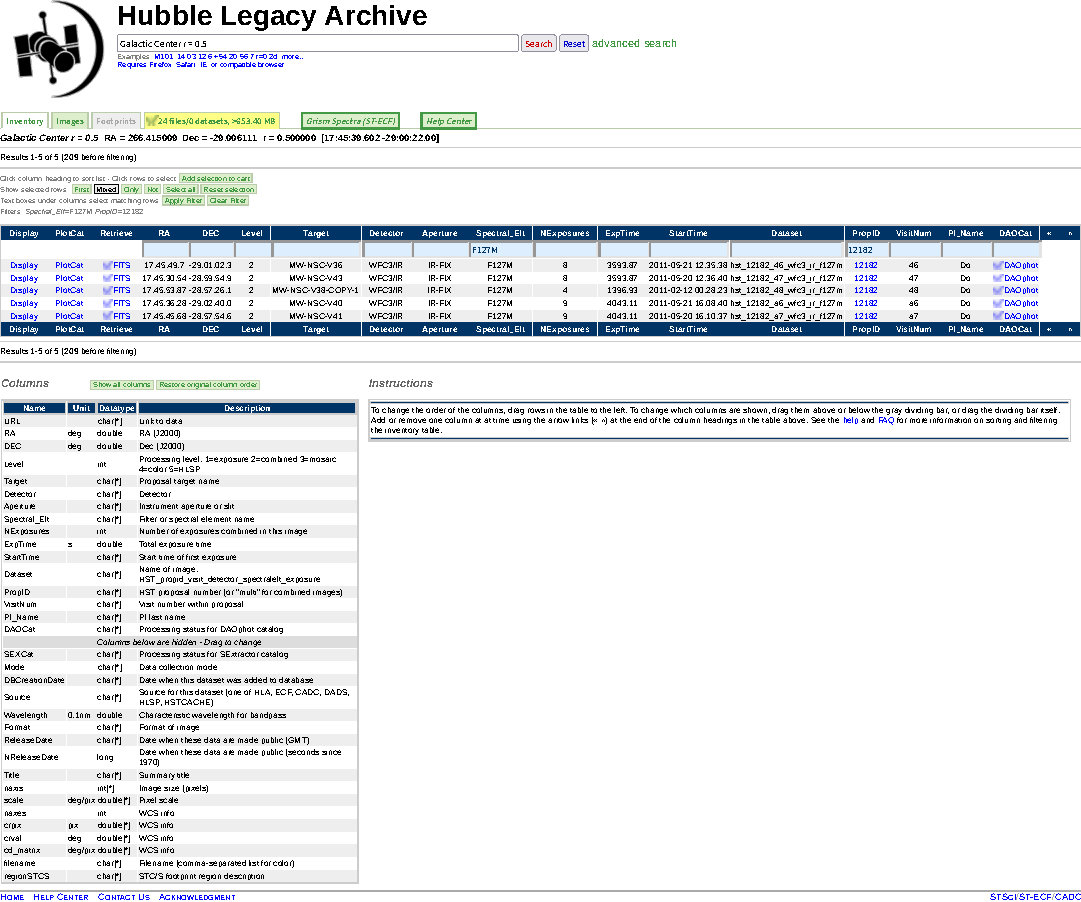
\includegraphics[width=\linewidth,page=1]{img/HLA_screenshot.pdf}
  \caption{Hubble Legacy Archive のスクリーンショット}
  \label{fig:screen:hla}
\end{figure}

\begin{table}
  \centering
  \caption{使用したデータの概要}
  \label{tab:data}
  \footnotesize
  \begin{tabular}{cccScc}
    \toprule
    \multicolumn{1}{c}{Filename}
    & \multicolumn{1}{c}{Object}
    & \multicolumn{1}{c}{Filter}
    & \multicolumn{1}{c}{$T_\text{exp}~(\unit{\s})$}
    & \multicolumn{1}{c}{Prop ID}
    & \multicolumn{1}{c}{PI name} \\
    \midrule
    \verb|hst_11671_04_wfc3_ir_f127m_run_1_drz|
    & ARCHES & F127M & 7190.786 & 11671 & Ghez \\
    \verb|hst_11671_04_wfc3_ir_f139m_run_1_drz|
    & ARCHES & F139M & 3492.327 & 11671 & Ghez \\
    \verb|hst_11671_05_wfc3_ir_f127m_run_1_drz|
    & QUINTUPLET & F127M & 7190.786 & 11671 & Ghez \\
    \verb|hst_11671_05_wfc3_ir_f139m_run_1_drz|
    & QUINTUPLET & F139M & 3492.327 & 11671 & Ghez \\
    \verb|hst_11671_06_wfc3_ir_f127m_run_1_drz|
    & SGRA & F127M & 7190.786 & 11671 & Ghez \\
    \verb|hst_11671_06_wfc3_ir_f139m_run_1_drz|
    & SGRA & F139M & 3492.327 & 11671 & Ghez \\
    \verb|hst_12182_46_wfc3_ir_f127m_run_1_drz|
    & MW-NSC-V35 & F127M & 3593.868 & 12182 & Do \\
    \verb|hst_12182_46_wfc3_ir_f139m_run_1_drz|
    & MW-NSC-V35 & F139M & 2193.086 & 12182 & Do \\
    \verb|hst_12182_47_wfc3_ir_f127m_run_1_drz|
    & MW-NSC-V43 & F127M & 3593.868 & 12182 & Do \\
    \verb|hst_12182_47_wfc3_ir_f139m_run_1_drz|
    & MW-NSC-V43 & F139M & 2193.086 & 12182 & Do \\
    \verb|hst_12182_48_wfc3_ir_f127m_run_1_drz|
    & MW-NSC-V38-COPY-1 & F127M & 1396.930 & 12182 & Do \\
    \verb|hst_12182_48_wfc3_ir_f139m_run_1_drz|
    & MW-NSC-V38-COPY-1 & F139M & 996.927 & 12182 & Do \\
    \verb|hst_12182_a6_wfc3_ir_f127m_run_1_drz|
    & MW-NSC-V37 & F127M & 4043.102 & 12182 & Do \\
    \verb|hst_12182_a6_wfc3_ir_f139m_run_1_drz|
    & MW-NSC-V37 & F139M & 2193.086 & 12182 & Do \\
    \verb|hst_12182_a7_wfc3_ir_f127m_run_1_drz|
     & MW-NSC-V41 & F127M & 4043.102 & 12182 & Do \\
    \verb|hst_12182_a7_wfc3_ir_f139m_run_1_drz|
    & MW-NSC-V41 & F139M & 1993.854 & 12182 & Do \\
        \bottomrule
  \end{tabular}
\end{table}

\subsection{Hubble Space Telescope/Wide Field Camera 3}
WFC3 の装置仕様はウェブ上に詳細なドキュメントが公開されている.\footnote{\url{https://hst-docs.stsci.edu/wfc3ihb}} WFC3 は紫外可視チャンネル (UVIS, two 2k${\times}$4k CCDs, $\ang{;;162}{\times}\ang{;;162}$, $\numrange{200}{1000}\,\si{\nano\meter}$) と赤外線チャンネル (1k${\times}$1k HgCdTe, $\ang{;;136}{\times}\ang{;;123}$, $\numrange{800}{1700}\,\si{\nano\meter}$) をもつ撮像分光観測装置である. HLA から取得したデータはバイアス引き, ダーク引き, フラット補正, バッドピクセル除去, 宇宙線除去, 非線形性補正, Drizzle による合成が完了している. また, FITS ファイルにはサイエンスフレームに加えてキャリブレーションの情報を保存したフレームも含まれている.

サイエンスフレームのカウント値は $\unit{electron\per\second}$ で与えられている. WFC3 の測光システムについてはドキュメントの \href{https://hst-docs.stsci.edu/wfc3dhb/chapter-9-wfc3-data-analysis/9-1-photometry}{9.1 Photometry} で詳細に記述されている. WFC3 の instrumental magnitude は以下の式で定義されている.
\begin{equation}
  m_\text{inst} = -2.5\log{F_\text{count}}.
  \label{eq:wfc3:instmag}
\end{equation}
$F_\text{count}$ はカウントレート ($\unit{electron\per\second}$) である. 物理的な値に変換するために WFC3 Instrument Science Report 2020-10 (\href{https://www.stsci.edu/files/live/sites/www/files/home/hst/instrumentation/wfc3/documentation/instrument-science-reports-isrs/_documents/2020/WFC3-ISR-2020-10.pdf}{Bajaj et al., 2020}) にて報告された等級原点を使用する. 表~\ref{tab:wfc3:zeromag} に今回使用するフィルタの等級原点と変換係数をリストした.

\begin{table}
  \centering
  \caption{HST/WFC3 等級原点リスト (WFC3 ISR 2020-10; Bajaj et al., 2020)}
  \label{tab:wfc3:zeromag}
  \begin{tabular}{ccccccc}
    \toprule
    \multicolumn{1}{c}{Filter}
    & \multicolumn{1}{c}{$\lambda_\text{pivot}$}
    & \multicolumn{1}{c}{$\Delta{\lambda}$}
    & \multicolumn{1}{c}{$M_\text{AB}$}
    & \multicolumn{1}{c}{$M_\text{Vega}$}
    & \multicolumn{1}{c}{$M_\text{ST}$}
    & \multicolumn{1}{c}{$F_{0,\lambda}{}^\star$} \\
    \midrule
    F127M & 12740.29 & 249.56 & 24.6246 & 23.6572 & 26.4584 & \num{9.452e-20} \\
    F139M & 13837.62 & 278.02 & 24.4663 & 23.3815 & 26.4796 & \num{9.313e-20} \\
    \bottomrule
    \multicolumn{7}{@{}l}{\footnotesize$^\star$: $\unit{electron\per\sec}$ から $\unit{erg\per\second\per\square\cm\per\angstrom}$ に変換するための係数.}
  \end{tabular}
\end{table}

\subsection{画像データ}
サンプルとして Arches の画像データを図~\ref{fig:11671:arches} に示した. 左右のパネルに \texttt{F127M} と \texttt{F139M} の画像をそれぞれリニアスケールで表示した. 画像のスケールはどちらも $\numrange{0.5}{2.5}\,\unit{electron\per\second}$ としている. その他の画像は図~\ref{fig:11671}, \ref{fig:12182a} に表示した. いずれの画像もピクセルスケールは $\SI{8.10e-3}{\square\arcsec}$ である. 画像の向きは ICRS 座標系準拠であり, 銀河座標系の座標軸を重ねている.

\begin{figure}
  \centering
  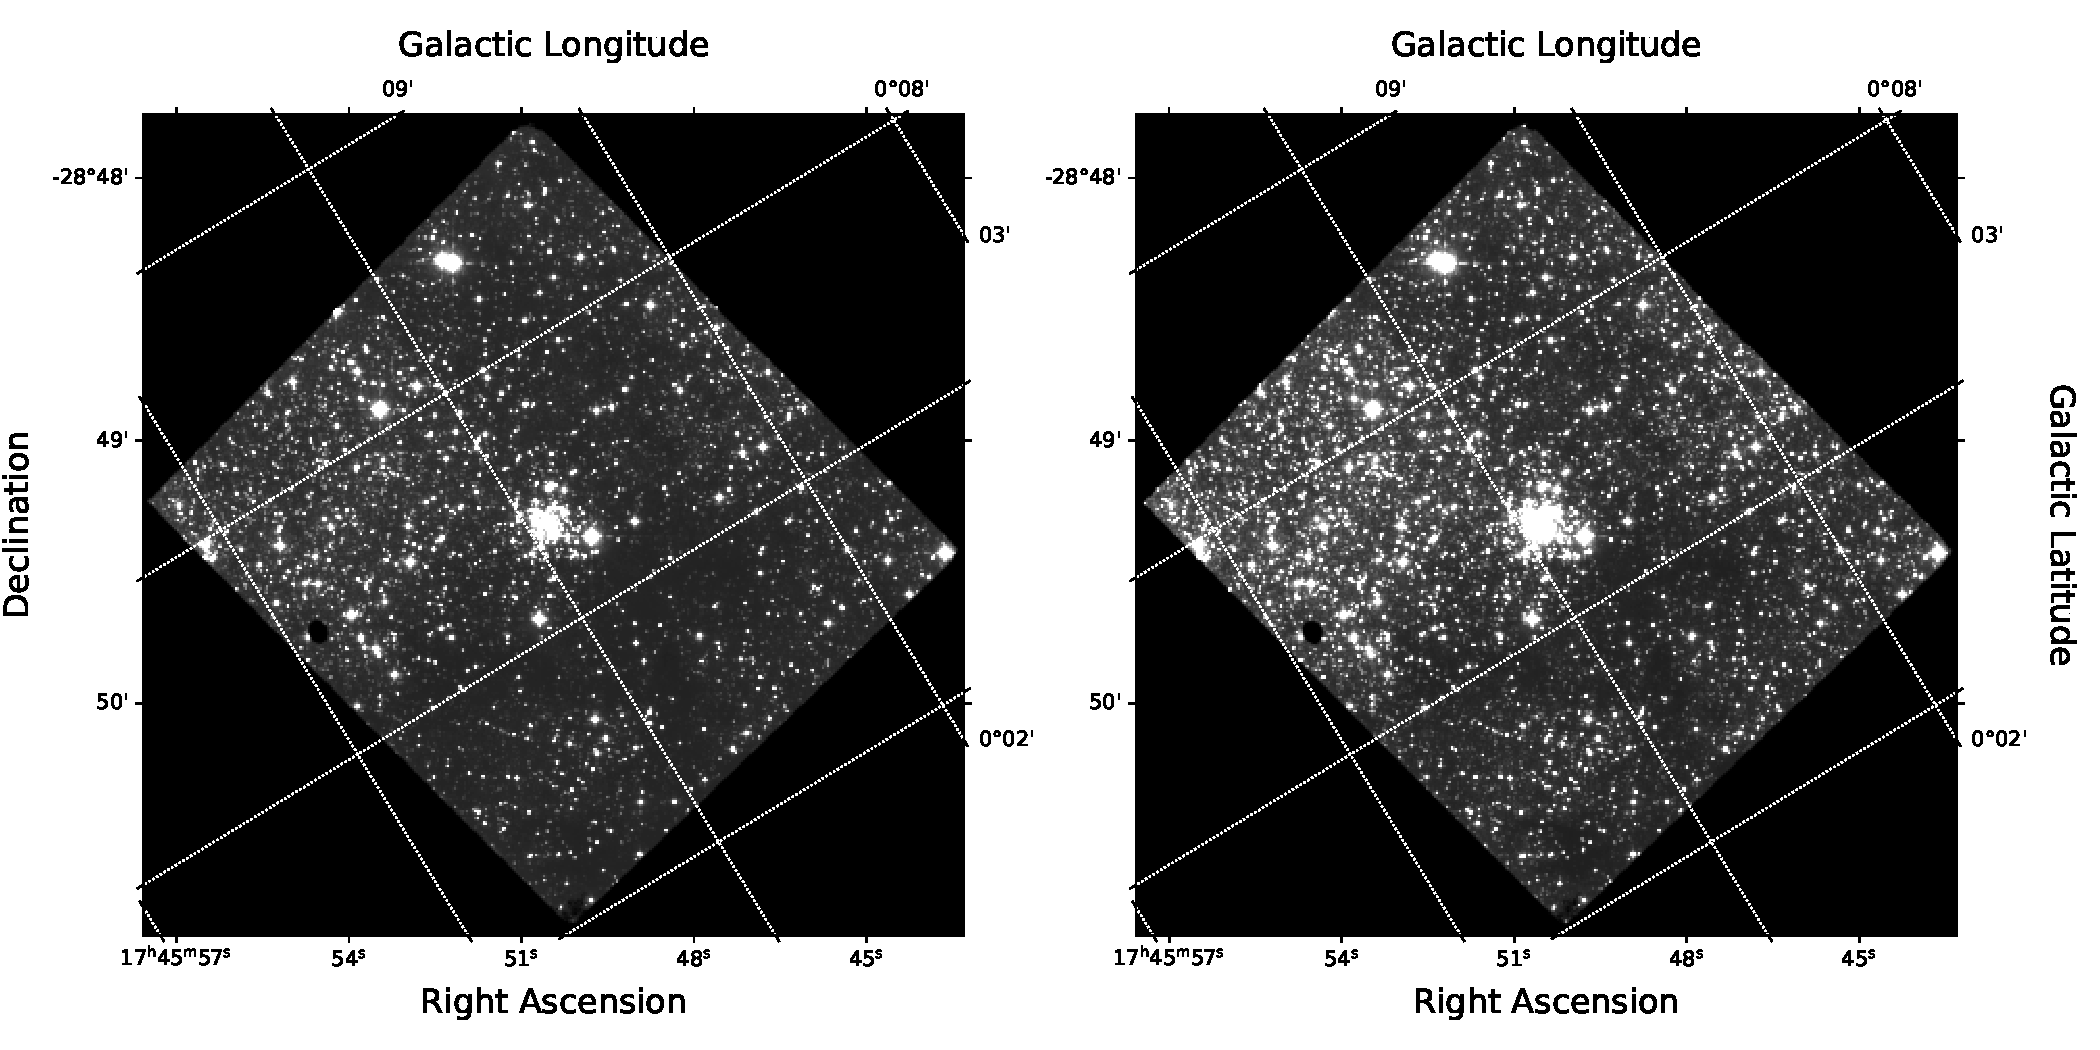
\includegraphics[width=\linewidth]{img/hst_11671_04_wfc3_ir_f127m_drz.pdf}
  \caption{Arches (Prop ID = 11671) の画像データ. 左パネルは \texttt{F127M} の画像, 右パネルは \texttt{F139M} の画像でどちらもリニアスケールで表示している.}
  \label{fig:11671:arches}
\end{figure}

\section{バックグラウンドレベルの評価}
有効画素のヒストグラムからバックグラウンドレベルを評価する. 選定した領域は星の密度が高い領域ではあるが, 総面積としては明るい星以外の領域が大半を占める. そこで画素値のヒストグラムを作成し, ピーク位置から典型的なバックグラウンド放射の強度を推定する.

表~\ref{tab:wfc3:zeromag} に記載された $F_{0,\lambda}$ (\texttt{PHOTFLAM}) を使用してカウント値をエネルギーフラックスに変換する.

\appendix
\section{画像データ}
この資料で使用した画像データを図~\ref{fig:11671}, \ref{fig:12182a} に表示する. 画像の表示の仕方はいずれも図~\ref{fig:11671:arches} と同様である.

\begin{figure}
  \centering
  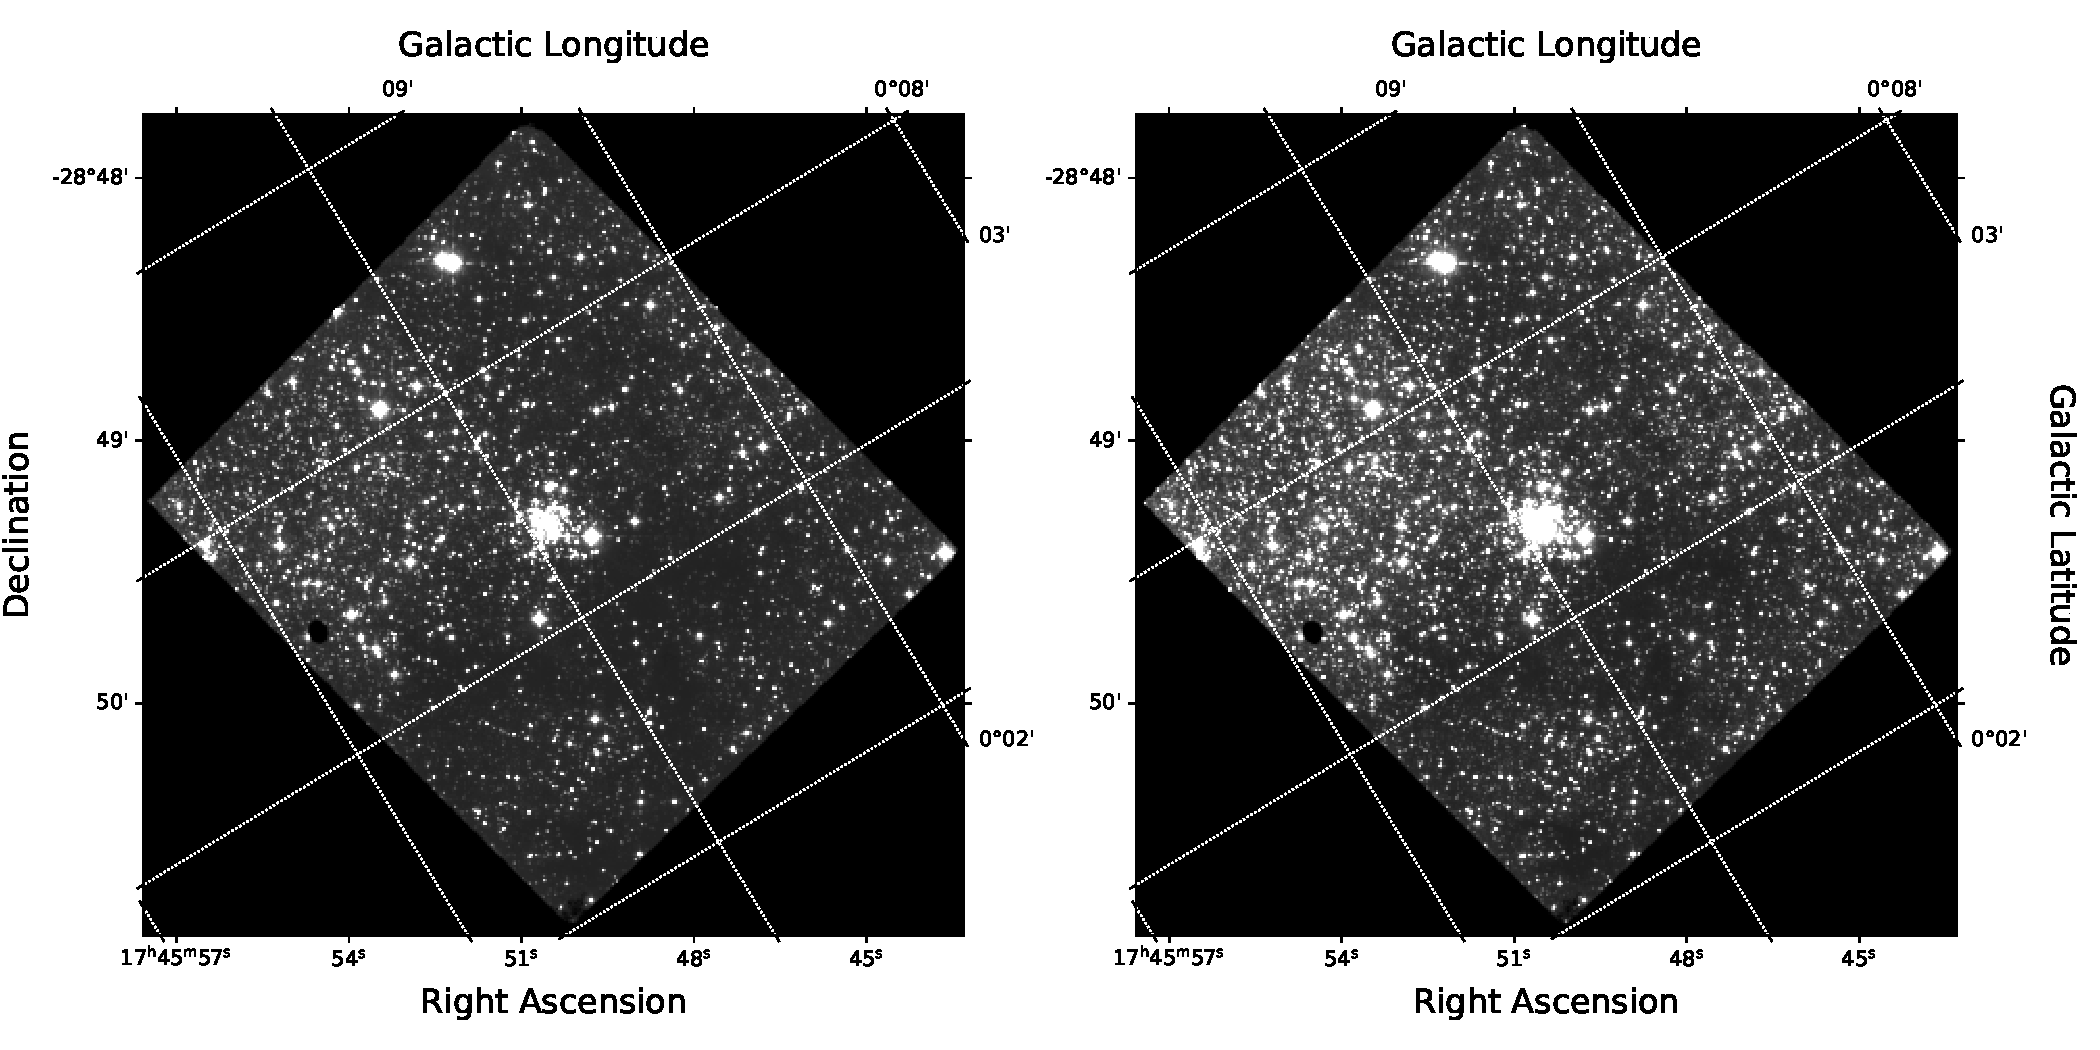
\includegraphics[width=\linewidth]{img/hst_11671_04_wfc3_ir_f127m_drz.pdf}
  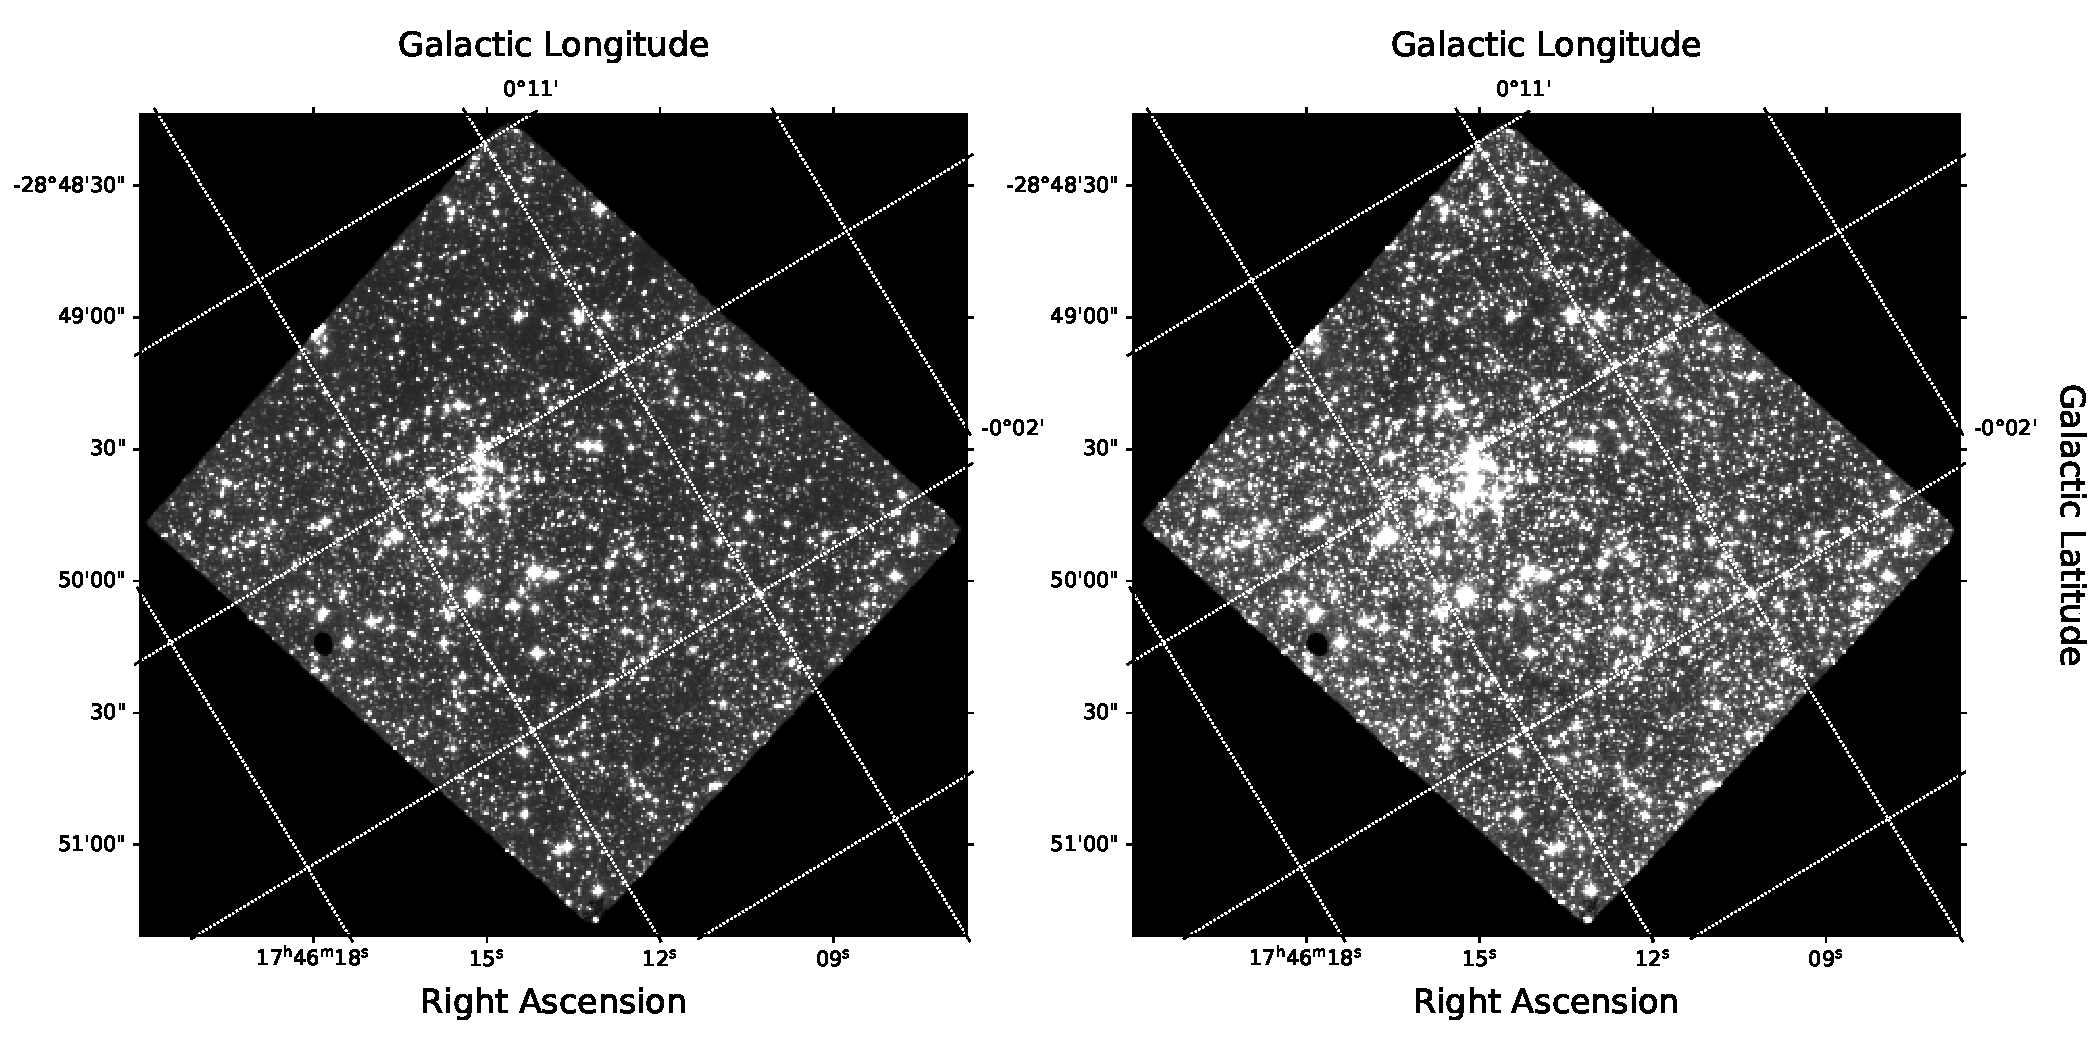
\includegraphics[width=\linewidth]{img/hst_11671_05_wfc3_ir_f127m_drz.pdf}
  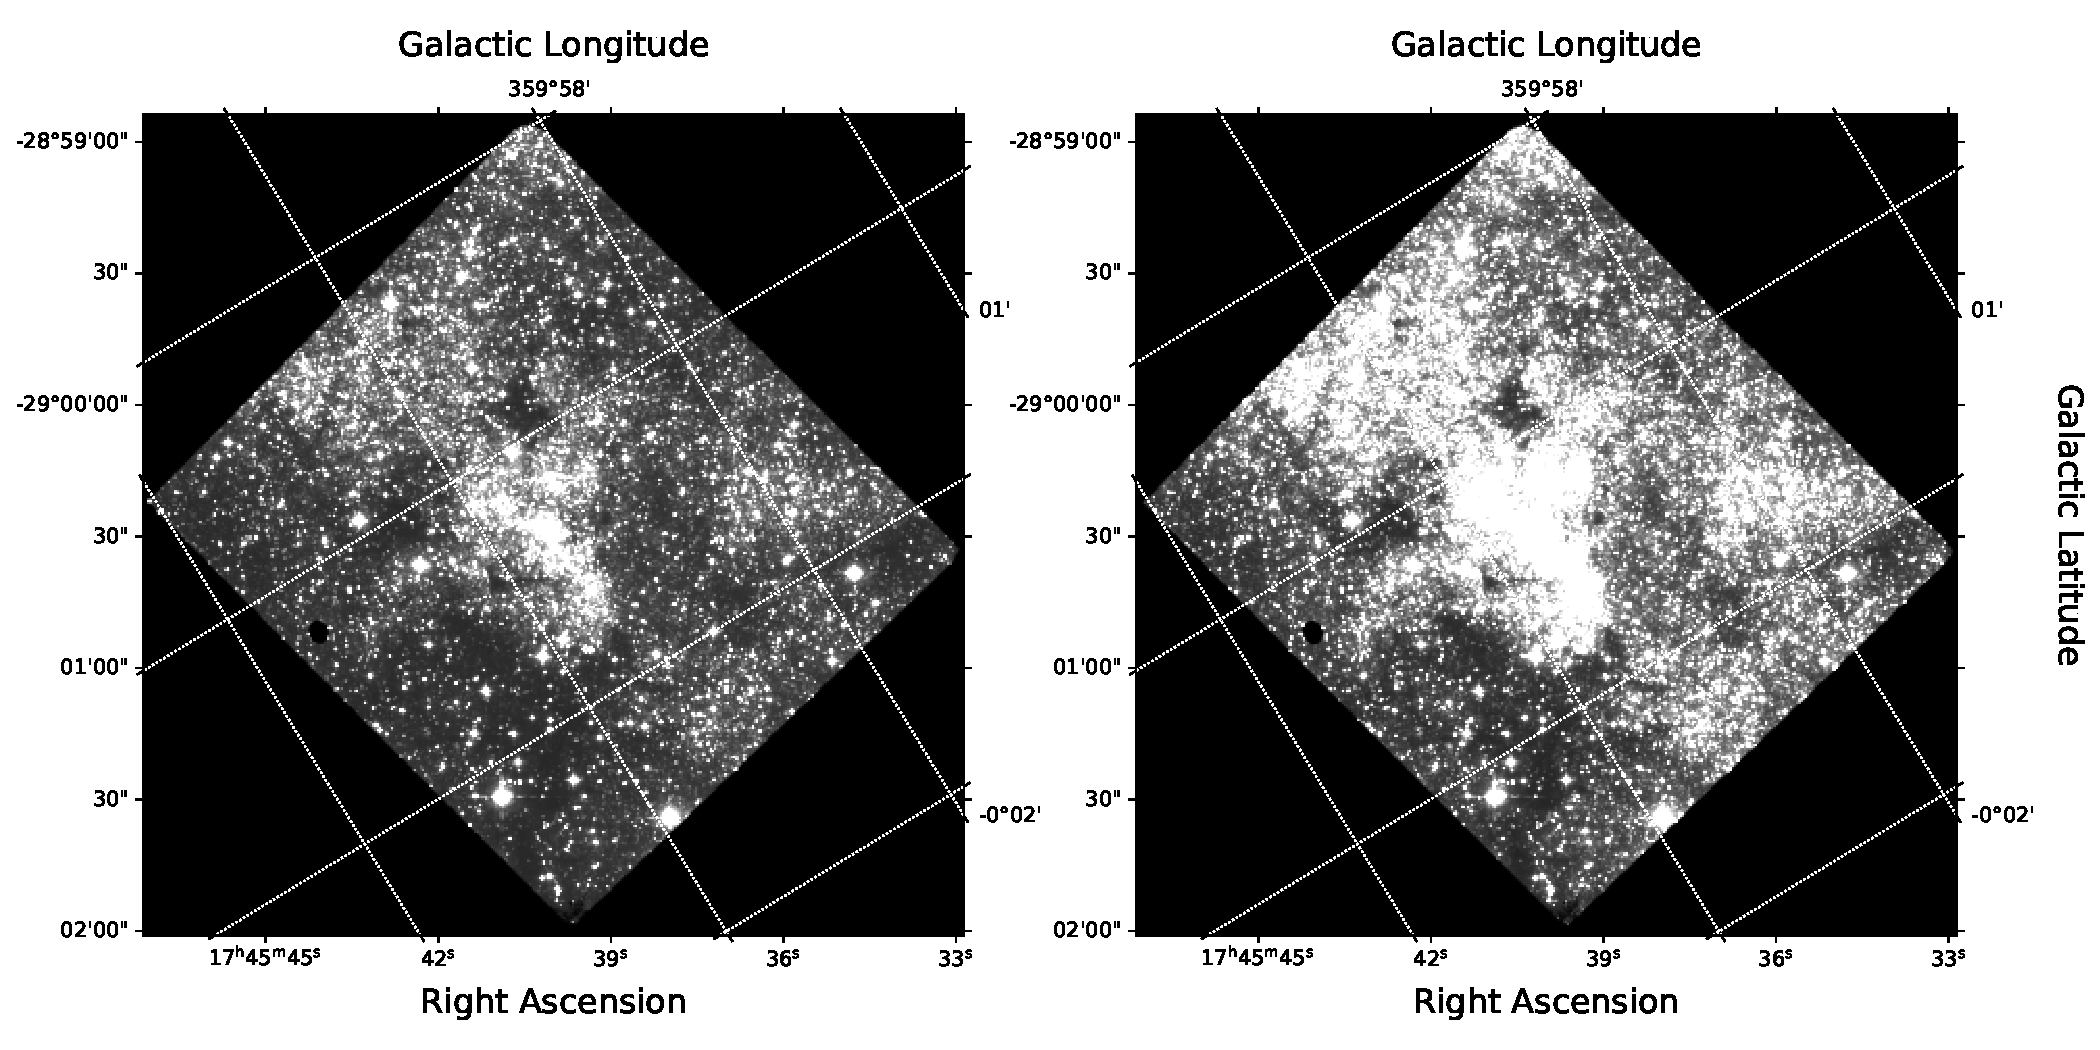
\includegraphics[width=\linewidth]{img/hst_11671_06_wfc3_ir_f127m_drz.pdf}
  \caption{Proposal ID 11671 の画像データ. 左パネルは \texttt{F127M} の画像, 右パネルは \texttt{F139M} の画像でどちらもリニアスケールで表示している. 上から順番に Arches, Quintuplet, SGRA の領域を示す.}
  \label{fig:11671}
\end{figure}

\begin{figure}
  \centering
  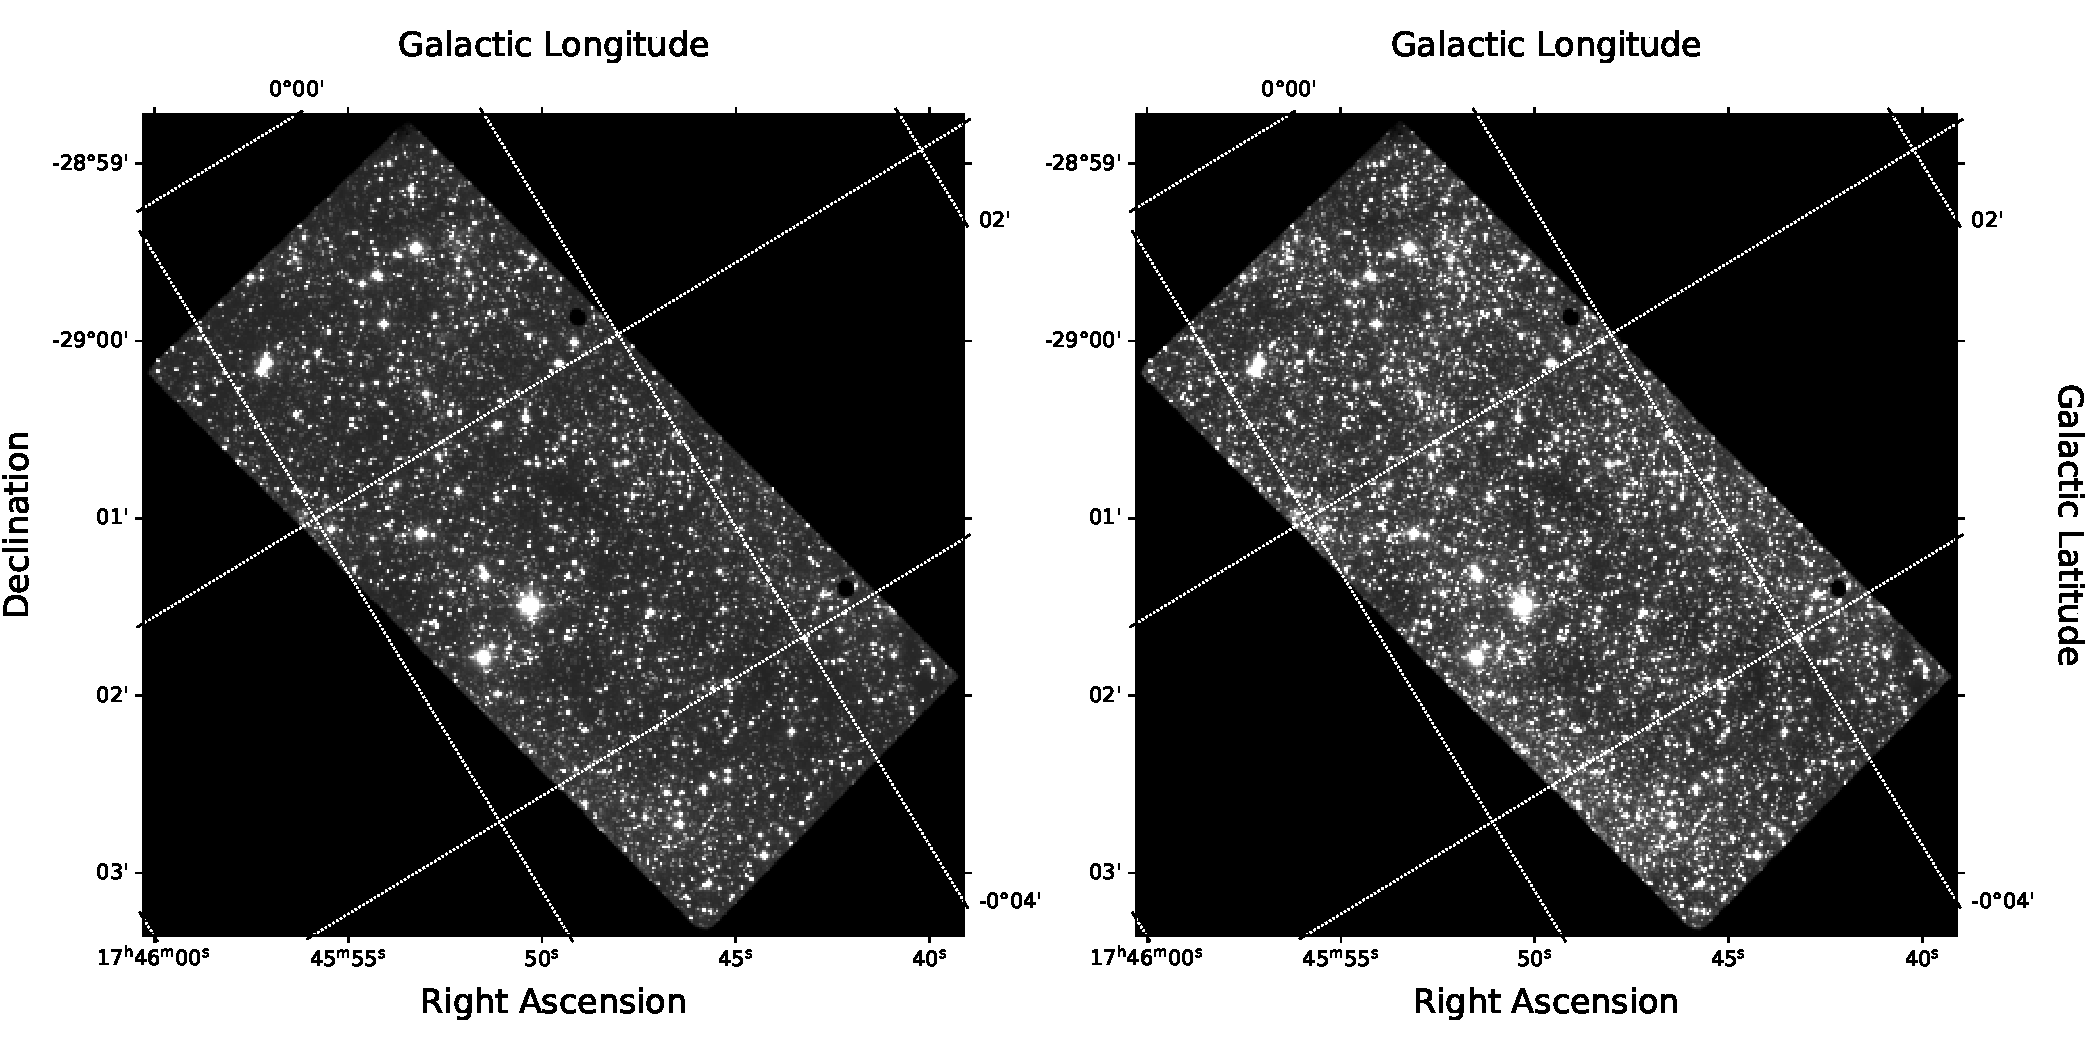
\includegraphics[width=\linewidth]{img/hst_12182_46_wfc3_ir_f127m_drz.pdf}
  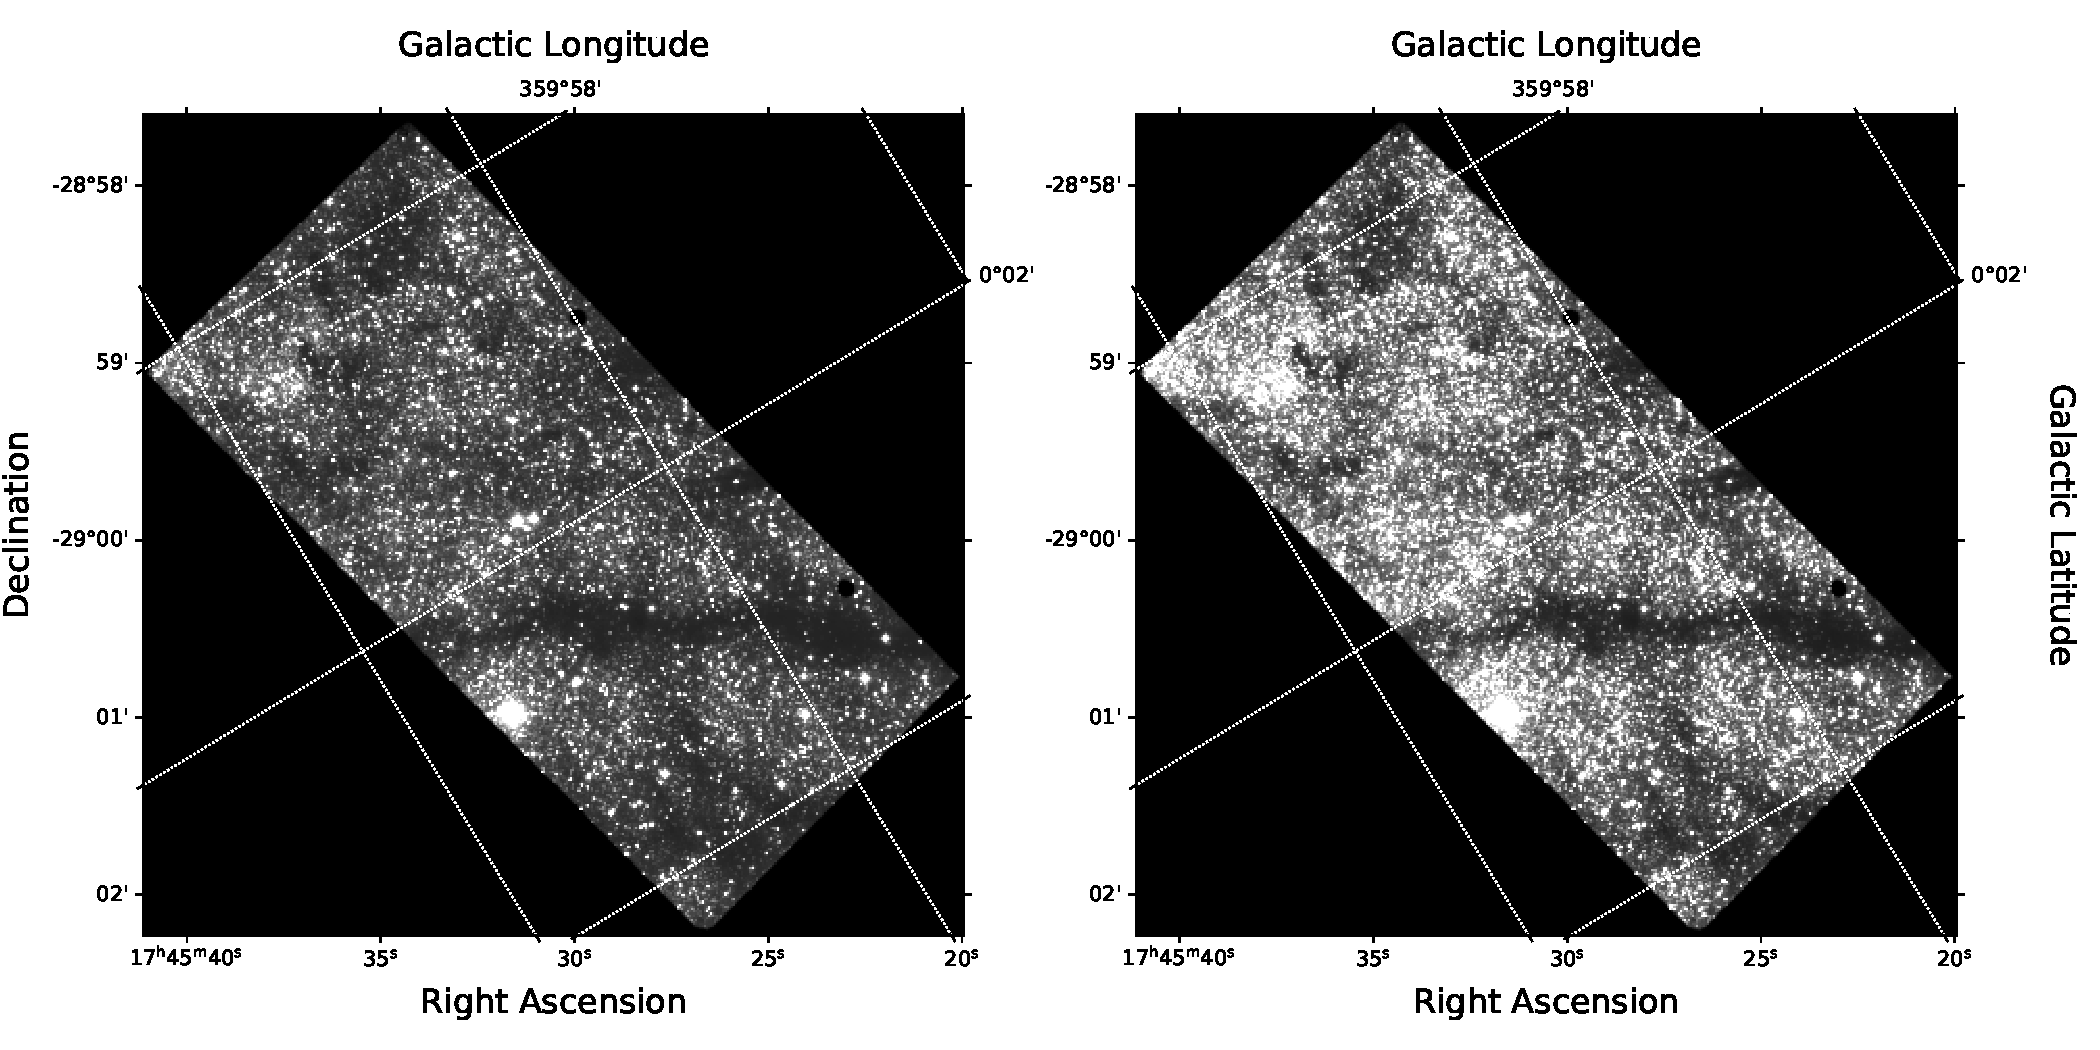
\includegraphics[width=\linewidth]{img/hst_12182_47_wfc3_ir_f127m_drz.pdf}
  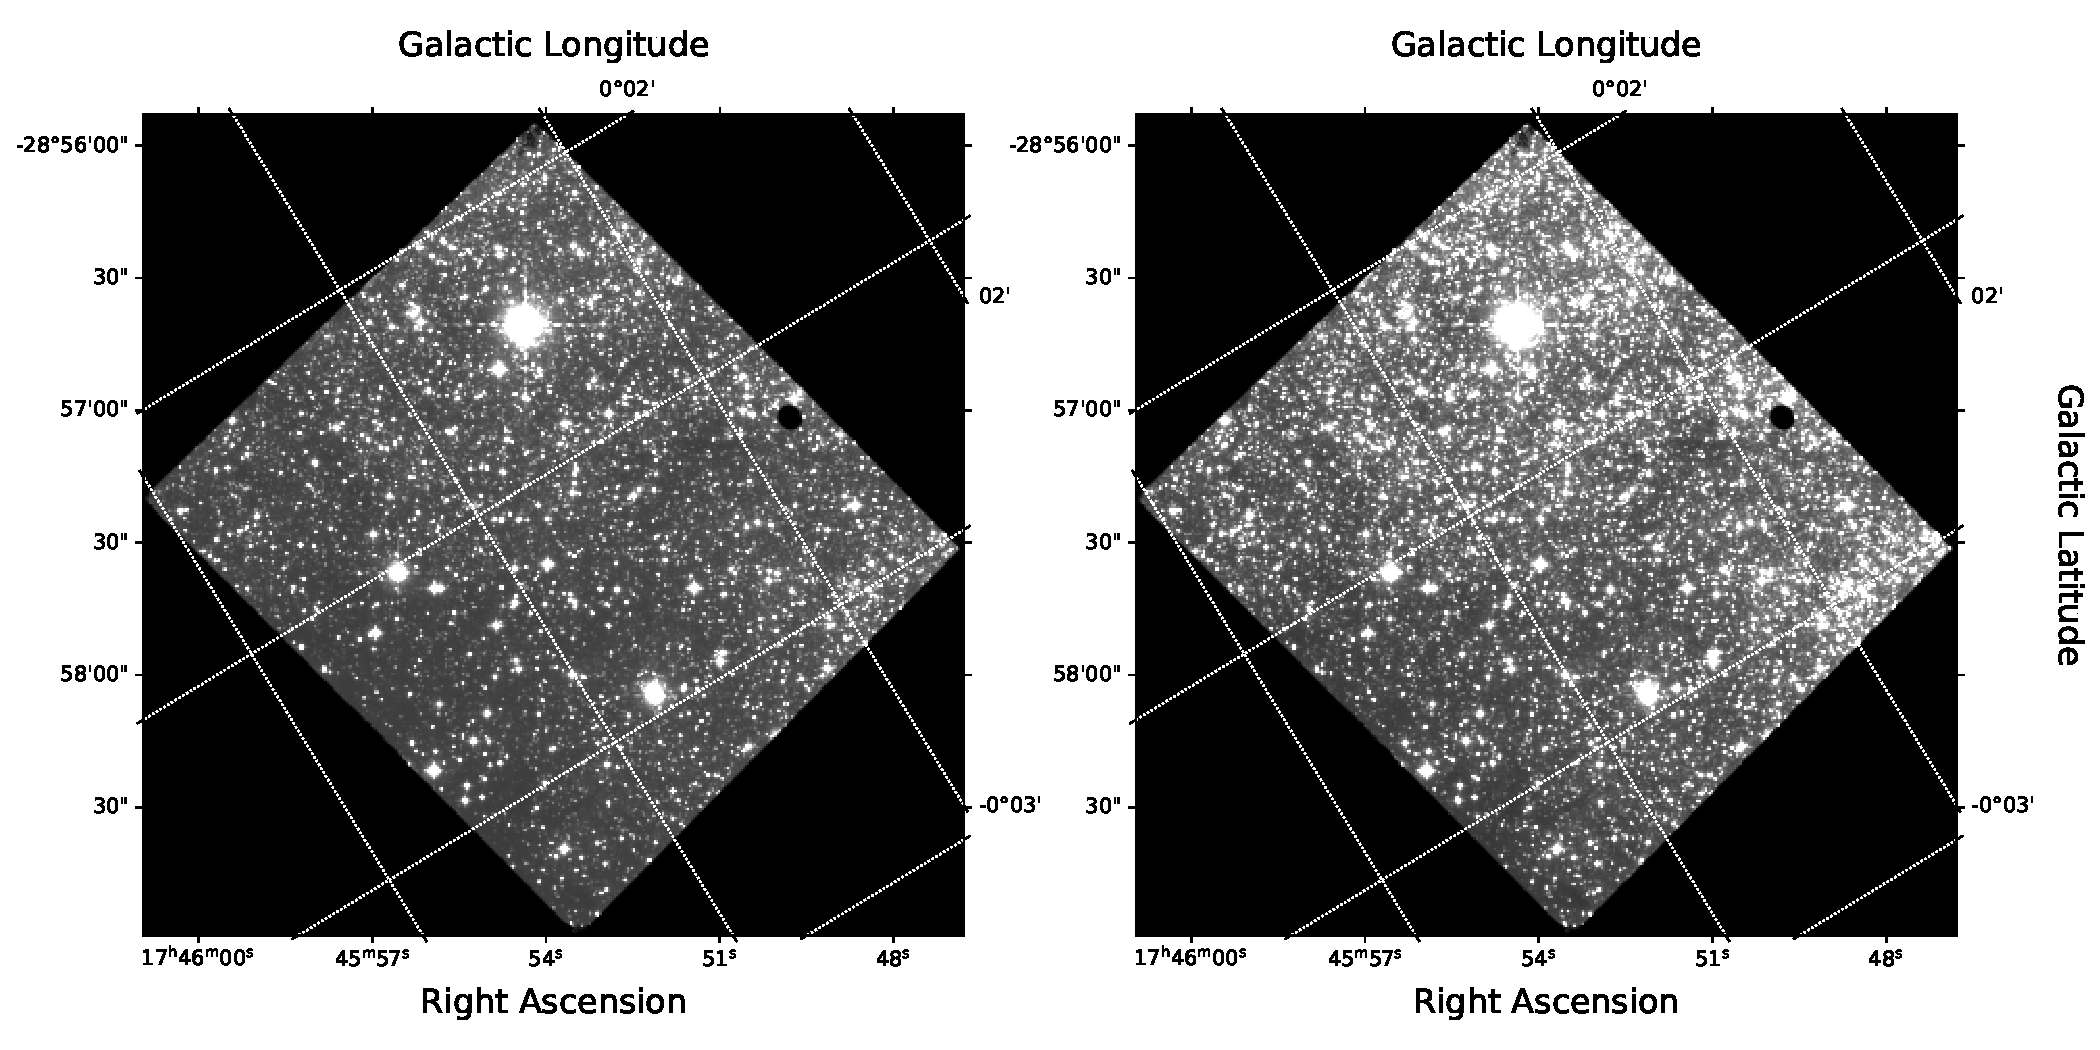
\includegraphics[width=\linewidth]{img/hst_12182_48_wfc3_ir_f127m_drz.pdf}
  \caption{Proposal ID 12182 の画像データ. 左パネルは \texttt{F127M} の画像, 右パネルは \texttt{F139M} の画像でどちらもリニアスケールで表示している. 上から順番に MW-NSC-V35, MW-NSC-V43, MW-NSC-V38-COPY-1 の領域を示す.}
  \label{fig:12182a}
\end{figure}

\addtocounter{figure}{-1}
\begin{figure}
  \centering
  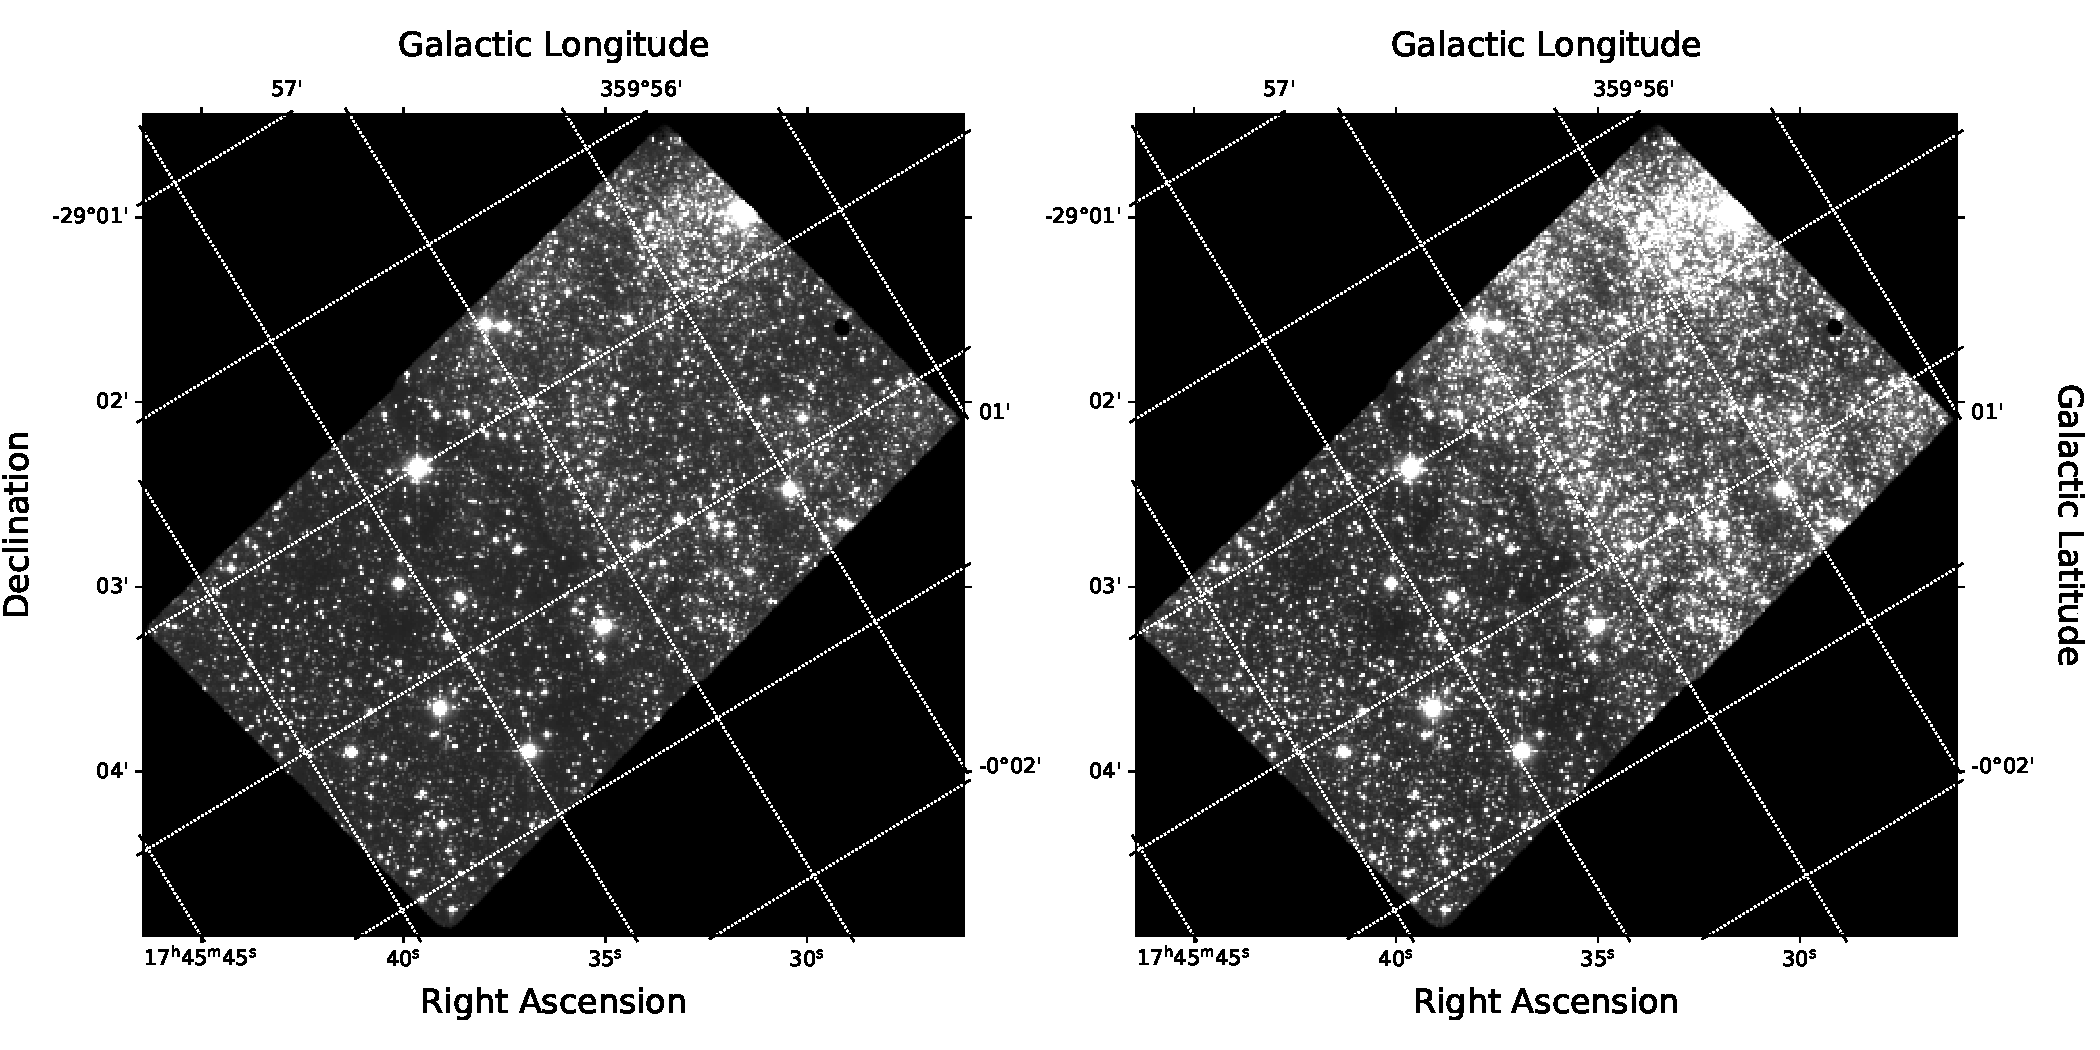
\includegraphics[width=\linewidth]{img/hst_12182_a6_wfc3_ir_f127m_drz.pdf}
  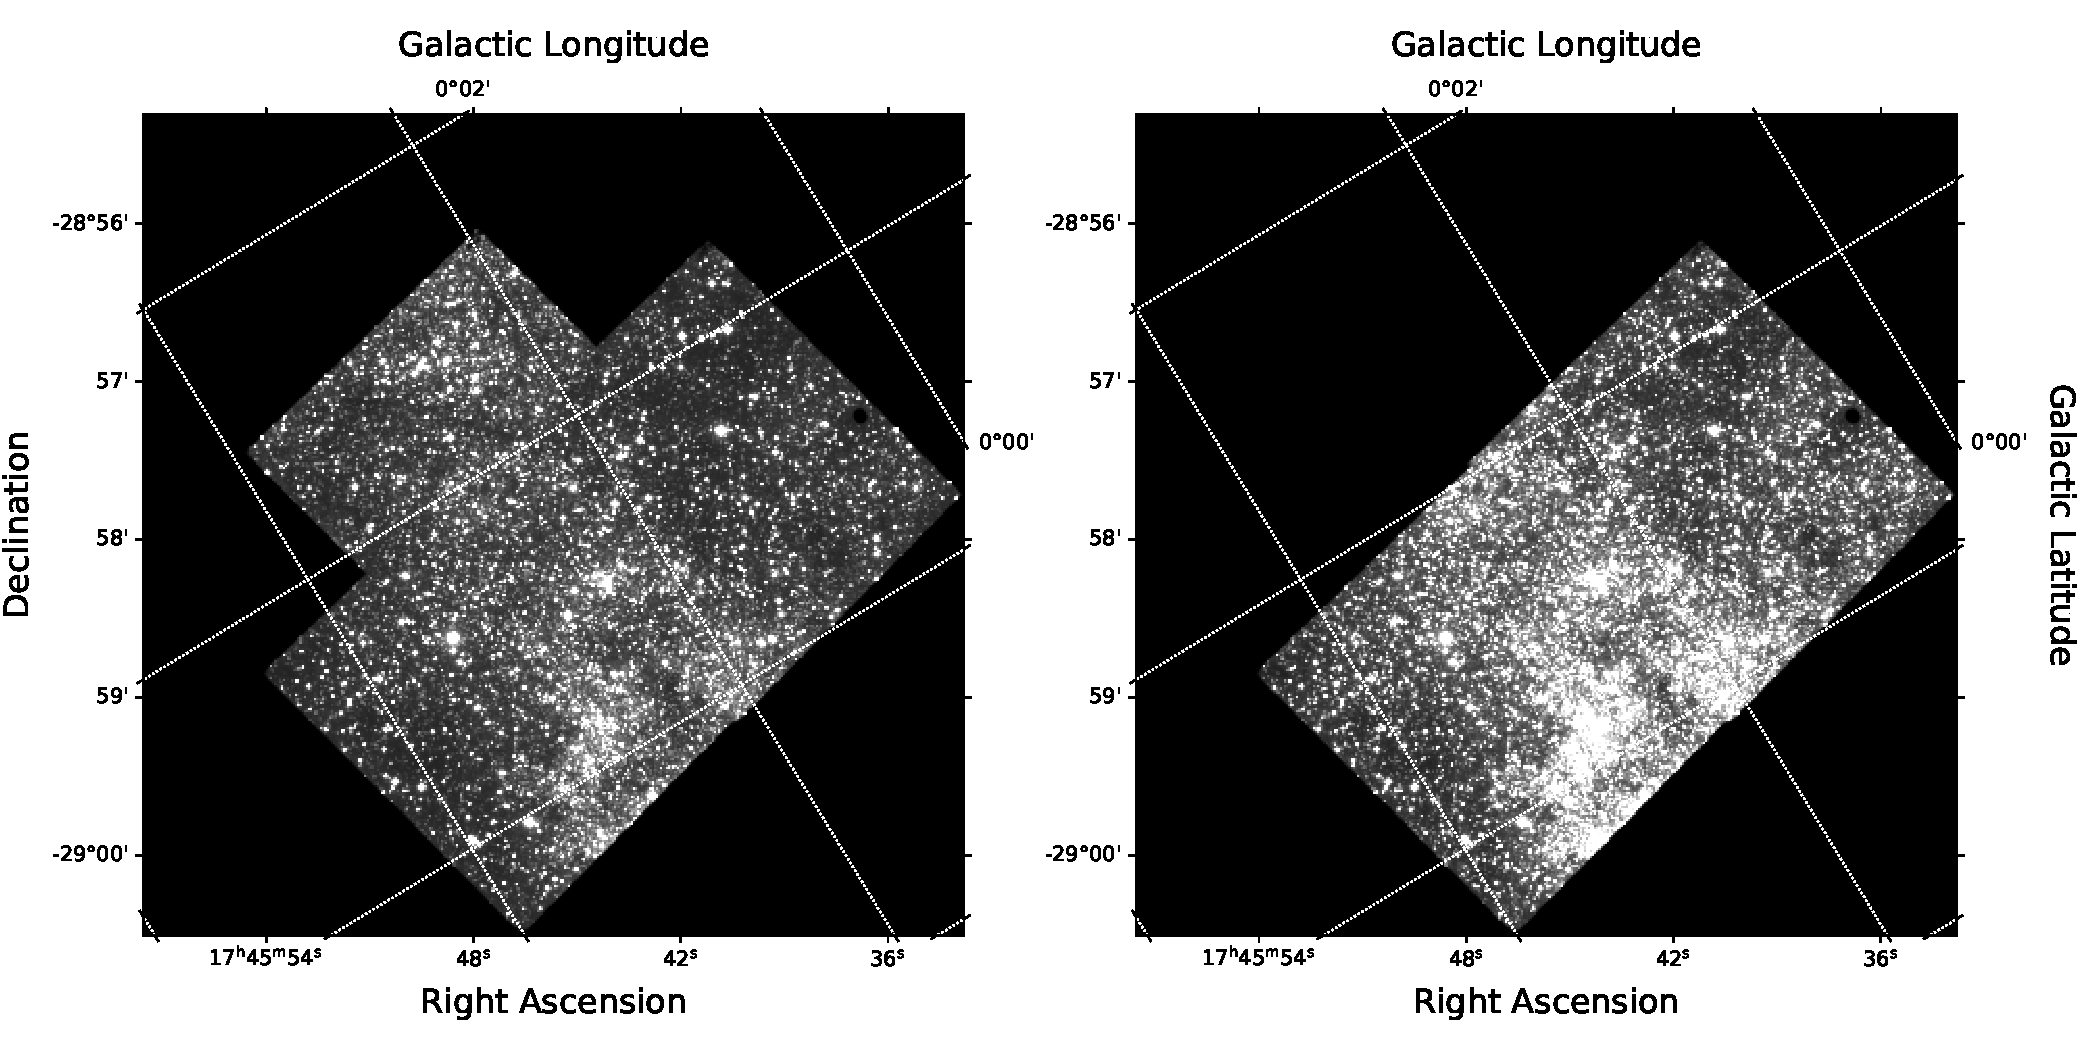
\includegraphics[width=\linewidth]{img/hst_12182_a7_wfc3_ir_f127m_drz.pdf}
  \caption{(\textit{cont.}) Proposal ID 12182 のデータ. 上から順番に MW-NSC-V37, MW-NSC-V41 の領域を示す.}
  \label{fig:12182b}
\end{figure}

\end{document}
